% =====================================================================
% Sections I, II, III.  \input{} from main.tex.
% =====================================================================

\section{Introduction}
\label{sec:intro}

A classifier deployed on a phone or a microcontroller is usually limited by
how much memory its weights occupy, not by how many multiplications the
processor can retire. Storage, over-the-air update size and the resident
footprint of a model all scale with its parameter count, which is why the
lightweight vision literature reports parameters first. That makes a specific
question the operative one: at a fixed parameter budget, which design extracts
the most accuracy? This paper answers it for low-resolution inputs by holding
parameters fixed, training every model under the same budget, and measuring
cost on real hardware instead of inferring it from operation counts.

Context Cluster \cite{coc} offers an unusual answer. Instead of attention or
convolution it mixes tokens by clustering them, and it reports competitive
accuracy at 5.3M parameters on $224\times224$ inputs. Its authors are explicit
that the goal is a new perspective on visual representation rather than state
of the art. What remains untested is whether the mechanism survives
compression: at one to three million parameters and $32\times32$ inputs, each
clustering stage sees few points, and the fold partitioning that keeps
clusters populated at high resolution has little left to partition. We treat
this as an open empirical question about operating regime, not as a criticism
of the original work.

To answer it we build a hybrid block in which each stage splits its channels
between a clustering branch and a local convolutional branch in ratio $\rho$,
and then vary one decision at a time: $\rho$, the fold partitioning, channel
shuffle, the stem stride, cluster occupancy, and the choice of local operator.
Every configuration trains for the same number of epochs on the same recipe,
repeats over three seeds, and is compared both with a Welch test on the seed
means and with an exact paired McNemar test on the $10{,}000$ test
predictions. Where a configuration has fewer than three seeds we say so in the
table.

The ablations point one way. Removing the local branch while holding the stem,
folds, depth and width fixed --- the comparison that isolates clustering from
everything it is usually bundled with --- costs $0.74$ pp. Removing the
clustering branch instead gains $1.03$ pp, at 10\% fewer parameters. Fold
partitioning and channel shuffle change accuracy by less than run-to-run
variation. The largest single effect in the whole study is the stem stride, at
$-5.72$ pp, and because stride~2 halves the resolution entering every
subsequent stage, most of that belongs to resolution rather than to anything
specific to clustering. At this scale the local branch carries the accuracy
and the clustering branch is a net cost.

Following that conclusion produces a design with no clustering in it at all.
Scaled to 2.71M parameters, given $7\times7$ depthwise kernels, and trained
with logit distillation, it reaches $61.21 \pm 0.40$ on Tiny-ImageNet. It
leads a parameter-matched ShuffleNetV2-x1.5 \cite{shufflenetv2} by $1.49$ pp
and its own ResNet-18 teacher by $2.46$ pp, both significant over seeds and
confirmed by a paired test on every seed individually. We chose
ShuffleNetV2-x1.5 as the primary baseline because an earlier version of our
model lost to it, and we report it rather than substituting something weaker.

Two caveats belong in the opening rather than buried later. The win holds
under distillation; with plain cross-entropy the margin over
ShuffleNetV2-x1.5 falls to $0.47$ pp and does not reach significance, and the
model merely ties its teacher. And the accuracy is bought with compute: at
matched parameters the proposed model performs $2.41\times$ the operations of
ShuffleNetV2-x1.5, though still $2.41\times$ fewer than the ResNet-18 it beats.

This paper contributes a controlled ablation of context clustering in the
lightweight low-resolution regime and the negative conclusion that it does not
pay for itself there; an all-local configuration that beats a
parameter-matched baseline and its own teacher on two datasets; a cost
protocol using graph-verified latency, per-batch-size memory reset and
weights reported separately from activations, together with the observation
that operation counts mispredict measured latency by more than fourfold; and
a release of every configuration, seed, per-image prediction and provenance
record behind the numbers.

% ---------------------------------------------------------------------
\section{Related Work}
\label{sec:related}

\textbf{Lightweight convolutional networks.} MobileNetV2 \cite{mobilenetv2}
established the inverted residual with a linear bottleneck, and ShuffleNetV2
\cite{shufflenetv2} argued that operation counts are a poor proxy for latency,
proposing four design rules derived from measured speed instead. Its channel
split, depthwise convolution and channel shuffle give a strong
accuracy-per-parameter trade-off, and the x1.5 width multiplier lands close to
the budget we study, which is why we adopt it as the primary baseline.
ConvNeXt \cite{convnext} later showed that widening depthwise kernels from
$3\times3$ to $7\times7$ buys roughly $0.7$ pp on ImageNet at negligible cost,
and RepLKNet \cite{replknet} pushed the idea further and attributed the gain
to effective receptive field rather than capacity. Our final design uses both
observations.

\textbf{Token mixers.} MetaFormer \cite{metaformer} separated the transformer
block into a token mixer and a channel MLP and showed that the surrounding
structure matters more than the mixer itself, which makes the mixer a clean
unit of ablation. Context Cluster \cite{coc} substitutes a clustering
operation: points are assigned to centres by similarity, aggregated, and
dispatched back. Reported results are at 5.3M parameters and $224\times224$.
We keep the MetaFormer skeleton fixed and vary only the mixer, which is what
lets a single number be attributed to clustering rather than to the
architecture around it.

\textbf{Knowledge distillation.} Hinton et al. \cite{hinton} match a student
to a teacher's softened logits, and the technique is routine in lightweight
vision because it closes part of the gap to a larger model at no inference
cost. Decoupled knowledge distillation \cite{dkd} separates the target and
non-target components of that loss and reweights them. A recurring difficulty
in comparisons is that distillation is often applied only to the proposed
model; we apply the identical recipe, teacher and seed to every student in
this paper, and report cross-entropy results alongside.

% ---------------------------------------------------------------------
\section{Methodology}
\label{sec:method}

\subsection{The hybrid block and its design space}

Every model in this study is built from the same four-stage MetaFormer
skeleton \cite{metaformer}. A block applies normalisation, a token mixer, a
LayerScale parameter and a stochastic-depth path, adds the residual, and
repeats the pattern with a channel MLP of ratio~3. Stages are separated by
stride-2 point reducers that halve resolution and widen the channel count.

The hybrid block parameterises the token mixer by a local ratio $\rho$. Given
$C$ input channels it routes $\rho C$ to a local convolutional branch and
$(1-\rho)C$ to a clustering branch, concatenates the two, and fuses them with
a $1\times1$ convolution; an optional channel shuffle precedes the split. The
clustering branch follows \cite{coc}: the feature map is divided into fold
tiles, centres are proposed within each tile, points are assigned to centres
by cosine similarity, aggregated, and dispatched back. Occupancy $r$, the
number of points per centre, is set by the proposal grid. Setting $\rho = 0$
recovers a pure clustering model and $\rho = 1$ removes clustering entirely,
which is what makes $\rho$ the variable the study turns on. Section~\ref{sec:ablation}
reports each of these knobs varied in isolation.

\begin{figure*}[!t]
\centering
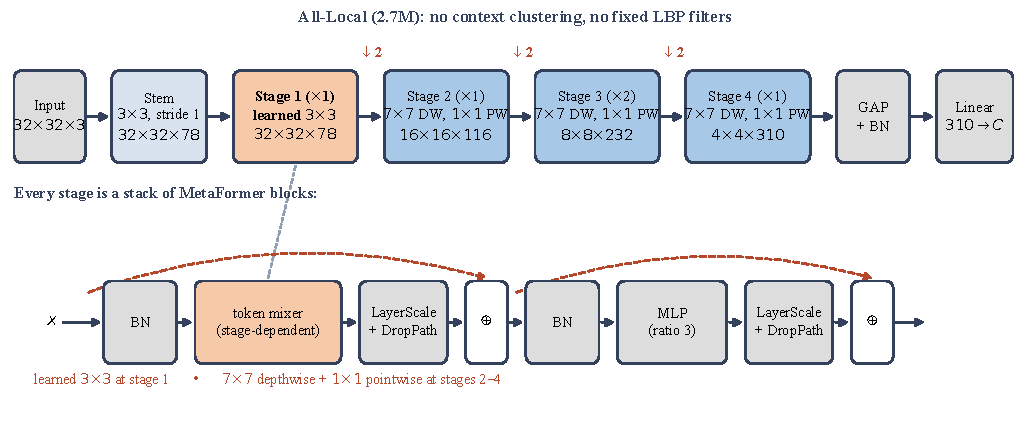
\includegraphics[width=\textwidth]{fig1_architecture.pdf}
\caption{The All-Local (2.7M) architecture. A stride-1 stem preserves the
$32\times32$ resolution into stage~1, whose token mixer is a learned
$3\times3$ convolution; stages~2--4 use $7\times7$ depthwise followed by
$1\times1$ pointwise convolution. Neither context clustering nor the fixed
LBP filters of the hybrid model appear in the final design.}
\label{fig:arch}
\end{figure*}

\subsection{The All-Local configuration}

The configuration the ablations select contains no clustering and no
hand-designed filters. Fig.~\ref{fig:arch} shows it.

The stem is a $3\times3$ convolution at stride~1, so stage~1 operates at the
full $32\times32$ resolution. This is the single most consequential choice in
the model: moving the stem to stride~2 costs $5.72$ pp
(Table~\ref{tab:ablation}), far more than any other decision we varied. At
$32\times32$ input there is little spatial information to discard, and
discarding half of it at the first layer is not recoverable downstream.

Stage~1 mixes tokens with a learned $3\times3$ convolution. The hybrid model
used fixed filters whose weights encode a sparse local binary pattern and
which expand the channel count eightfold before a pointwise projection;
Section~\ref{sec:ablation} shows that a plain learned convolution matches them
in accuracy at equal parameters while using $2.50\times$ less activation
memory, so we use the learned convolution.

Stages~2 to~4 mix tokens with a $7\times7$ depthwise convolution followed by a
$1\times1$ pointwise convolution. The wide kernel follows \cite{convnext}: with
only five blocks in the entire network, depth cannot grow the effective
receptive field, so each layer has to reach further, and a depthwise kernel
costs $k^2$ per channel rather than $C_\text{in}C_\text{out}k^2$. Widening
from $3\times3$ to $7\times7$ adds 35{,}600 parameters, 1.3\% of the model,
and 2.5M operations.

Channel widths are $[78, 116, 232, 310]$ with depths $[1, 1, 2, 1]$, giving
2{,}707{,}416 parameters with a 200-class head. The widths were chosen to
match ShuffleNetV2-x1.5 at 2{,}683{,}624 parameters so that the headline
comparison is at an equal budget; no other hyperparameter was tuned to the
baseline. A final normalisation, global average pooling and a linear
classifier complete the network.
